% !TeX program = xelatex
% HyperMem: Three-Layer Hypergraph Memory Architecture for AI Agents
% Compile: latexmk -xelatex hypermem-techreport.tex
% arXiv tech report — companion to "When Agents Remember, They Stop Building"

\documentclass[11pt, a4paper]{article}

% ═══════════════════════════════════════════════════════════
% PACKAGES
% ═══════════════════════════════════════════════════════════
\usepackage[top=25mm, bottom=28mm, left=25mm, right=25mm]{geometry}
\usepackage{fontspec}
\setmainfont{texgyrepagella-regular.otf}[
  BoldFont = texgyrepagella-bold.otf,
  ItalicFont = texgyrepagella-italic.otf,
  BoldItalicFont = texgyrepagella-bolditalic.otf,
]
\setsansfont{texgyreheros-regular.otf}[
  BoldFont = texgyreheros-bold.otf,
  ItalicFont = texgyreheros-italic.otf,
  Scale = 0.95,
]
\setmonofont{texgyrecursor-regular.otf}[
  BoldFont = texgyrecursor-bold.otf,
  Scale = 0.85,
]
\usepackage[protrusion=true]{microtype}
\usepackage{setspace}
\setstretch{1.15}
\setlength{\parindent}{0pt}
\setlength{\parskip}{0.5em}

\usepackage[dvipsnames,table]{xcolor}
\definecolor{deep}{RGB}{53,88,76}
\definecolor{accent}{RGB}{240,238,155}
\definecolor{faded}{RGB}{127,136,130}
\definecolor{subtle}{RGB}{238,235,225}
\definecolor{errcoral}{RGB}{255,107,128}
\definecolor{topicblue}{RGB}{70,130,180}
\definecolor{episodegreen}{RGB}{86,190,120}
\definecolor{factorange}{RGB}{230,160,60}

\usepackage{titlesec}
\titleformat{\section}{\sffamily\Large\bfseries\color{deep}}{\thesection}{0.7em}{}
\titleformat{\subsection}{\sffamily\large\color{deep}}{\thesubsection}{0.6em}{}
\titleformat{\subsubsection}{\sffamily\normalsize\itshape\color{faded}}{\thesubsubsection}{0.5em}{}

\usepackage{tikz}
\usetikzlibrary{arrows.meta, positioning, fit, calc, backgrounds, shapes.geometric, decorations.pathmorphing}
\usepackage{listings}
\usepackage{tabularray}
\UseTblrLibrary{booktabs}
\usepackage{adjustbox}
\usepackage{enumitem}
\setlist{nosep, leftmargin=1.5em}
\usepackage{float}
\usepackage{amsmath}
\usepackage{amssymb}
\usepackage{hyperref}
\hypersetup{colorlinks=true, linkcolor=deep, citecolor=deep, urlcolor=deep!70}

\lstdefinelanguage{TypeScript}{
  keywords={async, await, function, const, let, return, export, class, new, import, from, interface, type, extends, implements, if, else, throw, try, catch, typeof, public, private, readonly, Promise, string, number, boolean, unknown, void, true, false, null, undefined},
  morecomment=[l]{//},
  morecomment=[s]{/*}{*/},
  morestring=[b]',
  morestring=[b]",
  morestring=[b]`,
  sensitive=true,
}
\lstset{
  language=TypeScript,
  basicstyle=\ttfamily\small,
  keywordstyle=\bfseries\color{deep},
  commentstyle=\itshape\color{faded},
  stringstyle=\color{deep!60},
  backgroundcolor=\color{subtle!50},
  frame=single,
  rulecolor=\color{deep!20},
  framesep=6pt,
  xleftmargin=6pt,
  xrightmargin=6pt,
  breaklines=true,
  showstringspaces=false,
  tabsize=2,
  captionpos=b,
  aboveskip=8pt,
  belowskip=8pt,
}

% ═══════════════════════════════════════════════════════════
% TITLE
% ═══════════════════════════════════════════════════════════
\title{%
  \sffamily\bfseries
  HyperMem: Three-Layer Hypergraph Memory\\
  Architecture for AI Agents%
}
\author{%
  Hengyuan Zhu\\
  {\small University of South Carolina}\\
  {\small\texttt{hengyuaz@email.sc.edu}}%
}
\date{April 2026}

\begin{document}
\maketitle

\begin{abstract}
\noindent
Existing memory systems for conversational AI agents rely on flat retrieval-augmented generation (RAG) or pairwise knowledge graphs, both of which fragment temporally dispersed information and lose higher-order relational structure.
We present an analysis of \textbf{HyperMem}~[1], a three-layer hypergraph memory architecture that organizes long-term conversational memory into \emph{Topic}, \emph{Episode}, and \emph{Fact} layers connected by hyperedges---edges that link arbitrary subsets of nodes rather than pairs alone.
A coarse-to-fine retrieval pipeline traverses these layers (Topic $\to$ Episode $\to$ Fact), achieving \textbf{92.73\%} accuracy on the LoCoMo benchmark (+6.24\% over the previous best RAG method) while requiring only \textbf{7.5$\times$} the token budget of a minimal baseline, compared to 35.3$\times$ for GraphRAG.
We contextualize HyperMem within the EverOS production API~[2] that engineers this architecture into physically isolated memory spaces, and connect the memory retrieval quality to downstream agent behavioral findings from a companion $2 \times 2$ factorial study~[3] where memory is associated with $\eta^2 = .917$ of behavioral variance.
\end{abstract}

% ═══════════════════════════════════════════════════════════
% §1 INTRODUCTION
% ═══════════════════════════════════════════════════════════
\section{Introduction}

Long-term memory is a prerequisite for AI agents that must maintain coherent behavior across extended interactions. Existing approaches fall short: \textbf{RAG} methods (75.48\%--86.49\% on LoCoMo~[4]) are limited by pairwise edges that fragment many-to-many conversational relationships, while \textbf{agent memory systems} like Mem0~[7] (76.02\%) and MemGPT~[9] lack structured mechanisms connecting facts to temporal episodes and thematic topics.

HyperMem~[1] addresses these limitations with: (1) a \textbf{three-layer hypergraph} $H = (V^T \cup V^E \cup V^F,\; E^E \cup E^F)$ where hyperedges preserve higher-order associations that pairwise graphs discard; (2) a \textbf{coarse-to-fine retrieval pipeline} yielding 7.5$\times$ token efficiency vs.\ 35.3$\times$ for GraphRAG; and (3) \textbf{SOTA results} on LoCoMo: 92.73\% overall (+6.24\% over HyperGraphRAG~[6]), with strong multi-hop (93.62\%) and temporal reasoning (89.72\%).

This report describes HyperMem's architecture and results, examines how EverOS~[2] engineers it into production, and connects memory retrieval quality to downstream agent behavior from a companion factorial study~[3].

% ═══════════════════════════════════════════════════════════
% §2 ARCHITECTURE
% ═══════════════════════════════════════════════════════════
\section{Architecture}

\subsection{Hypergraph Formalization}

HyperMem's memory is a weighted hypergraph:
\begin{equation}
  H = (V^T \cup V^E \cup V^F,\; E^E \cup E^F)
\end{equation}
The three node sets are: $V^T$ (\textbf{Topic}---thematic aggregates across time), $V^E$ (\textbf{Episode}---temporally contiguous dialogue segments with transcript, title, summary), and $V^F$ (\textbf{Fact}---atomic queryable assertions with content, potential queries, keywords). Two hyperedge sets connect them: $E^E$ links each topic to its constituent episodes $\{v^E_1, \ldots, v^E_k\}$ with weights $w^E$, and $E^F$ links each episode to its facts $\{v^F_1, \ldots, v^F_m\}$ with weights $w^F$. Unlike pairwise edges, each hyperedge connects a \emph{set} of nodes simultaneously---a single topic hyperedge can unify seven match discussions scattered across ten months, precisely the aggregation that pairwise approaches fragment.

\subsection{Three-Layer Structure}

\begin{figure}[H]
\centering
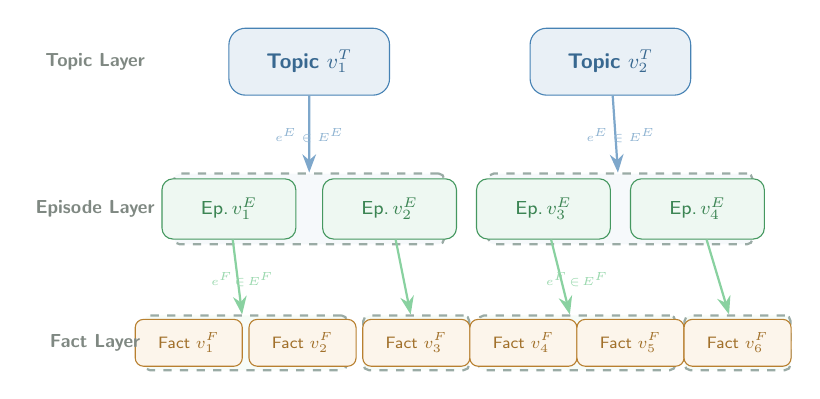
\begin{tikzpicture}[scale=0.85, every node/.style={scale=0.85},
  >=Stealth,
  topic/.style={
    rectangle, rounded corners=6pt,
    draw=topicblue, fill=topicblue!12,
    minimum width=24mm, minimum height=10mm,
    font=\sffamily\small\bfseries, text=topicblue!80!black,
  },
  episode/.style={
    rectangle, rounded corners=4pt,
    draw=episodegreen!80!black, fill=episodegreen!10,
    minimum width=20mm, minimum height=9mm,
    font=\sffamily\footnotesize, text=episodegreen!70!black,
  },
  fact/.style={
    rectangle, rounded corners=3pt,
    draw=factorange!80!black, fill=factorange!10,
    minimum width=16mm, minimum height=7mm,
    font=\sffamily\scriptsize, text=factorange!70!black,
  },
  hedge/.style={
    draw=deep!50, thick, rounded corners=2pt, dashed,
  },
  arr/.style={
    ->, thick, color=deep!60,
  },
  layerlabel/.style={
    font=\sffamily\footnotesize\bfseries, text=faded,
  },
]

% --- Topic Layer ---
\node[topic] (t1) at (0, 0) {Topic $v^T_1$};
\node[topic] (t2) at (4.5, 0) {Topic $v^T_2$};
\node[layerlabel] at (-3.2, 0) {Topic Layer};

% --- Episode Layer ---
\node[episode] (e1) at (-1.2, -2.2) {Ep.\,$v^E_1$};
\node[episode] (e2) at (1.2, -2.2) {Ep.\,$v^E_2$};
\node[episode] (e3) at (3.5, -2.2) {Ep.\,$v^E_3$};
\node[episode] (e4) at (5.8, -2.2) {Ep.\,$v^E_4$};
\node[layerlabel] at (-3.2, -2.2) {Episode Layer};

% --- Fact Layer ---
\node[fact] (f1) at (-1.8, -4.2) {Fact $v^F_1$};
\node[fact] (f2) at (-0.1, -4.2) {Fact $v^F_2$};
\node[fact] (f3) at (1.6, -4.2) {Fact $v^F_3$};
\node[fact] (f4) at (3.2, -4.2) {Fact $v^F_4$};
\node[fact] (f5) at (4.8, -4.2) {Fact $v^F_5$};
\node[fact] (f6) at (6.4, -4.2) {Fact $v^F_6$};
\node[layerlabel] at (-3.2, -4.2) {Fact Layer};

% --- Hyperedges (Topic -> Episodes) ---
\begin{scope}[on background layer]
  \node[hedge, fill=topicblue!5, inner sep=4pt,
        fit=(e1)(e2)] (he1) {};
  \node[hedge, fill=topicblue!5, inner sep=4pt,
        fit=(e3)(e4)] (he2) {};
\end{scope}
\draw[arr, topicblue!70] (t1) -- (he1);
\draw[arr, topicblue!70] (t2) -- (he2);

% --- Hyperedges (Episode -> Facts) ---
\begin{scope}[on background layer]
  \node[hedge, fill=episodegreen!5, inner sep=3pt,
        fit=(f1)(f2)] (hf1) {};
  \node[hedge, fill=episodegreen!5, inner sep=3pt,
        fit=(f3)] (hf2) {};
  \node[hedge, fill=episodegreen!5, inner sep=3pt,
        fit=(f4)(f5)] (hf3) {};
  \node[hedge, fill=episodegreen!5, inner sep=3pt,
        fit=(f6)] (hf4) {};
\end{scope}
\draw[arr, episodegreen!70] (e1) -- (hf1);
\draw[arr, episodegreen!70] (e2) -- (hf2);
\draw[arr, episodegreen!70] (e3) -- (hf3);
\draw[arr, episodegreen!70] (e4) -- (hf4);

% --- Hyperedge labels ---
\node[font=\sffamily\tiny, text=topicblue!60] at (0, -1.1) {$e^E \in E^E$};
\node[font=\sffamily\tiny, text=topicblue!60] at (4.65, -1.1) {$e^E \in E^E$};
\node[font=\sffamily\tiny, text=episodegreen!60] at (-1.0, -3.25) {$e^F \!\in\! E^F$};
\node[font=\sffamily\tiny, text=episodegreen!60] at (4.0, -3.25) {$e^F \!\in\! E^F$};

\end{tikzpicture}
\caption{HyperMem three-layer hypergraph. Dashed boxes are hyperedges connecting parent nodes to \emph{sets} of children. Topic layer aggregates across time; Episode layer preserves temporal continuity; Fact layer stores atomic assertions.}
\label{fig:architecture}
\end{figure}

\subsection{Construction Pipeline}

The hypergraph is built in three streaming stages. \textbf{(1) Episode Detection}: an LLM-driven boundary detector segments dialogue based on semantic completeness, temporal gaps, and topic-shift signals, producing (transcript, title, summary) triples. \textbf{(2) Topic Aggregation}: a streaming aggregator assigns episodes to topics (initialize, create, or update) with contribution weights $w^E$. \textbf{(3) Fact Extraction}: atomic facts are extracted per episode, each storing (content, potential\_queries, keywords). The \texttt{potential\_queries} field pre-generates likely query patterns---reminiscent of HyDE~[10]---transforming passive matching into active query alignment.

\subsection{Embedding Propagation}

Dual indexing combines BM25 with dense embeddings (Qwen3-Embedding-4B). A non-parametric one-step propagation transfers structural information:
\begin{equation}
  \mathbf{h}_e = \sum_{v \in e} w_v \cdot \mathbf{h}_v \;,\qquad
  \mathbf{h}'_v = \mathbf{h}_v + \lambda \sum_{e \ni v} \mathbf{h}_e \quad (\lambda = 0.5)
\end{equation}
No learned weights or iterative message passing---deliberately conservative to avoid over-smoothing. The $\lambda = 0.5$ balances original semantic content with structural context.

% ═══════════════════════════════════════════════════════════
% §3 RETRIEVAL PIPELINE
% ═══════════════════════════════════════════════════════════
\section{Retrieval Pipeline}

\subsection{Coarse-to-Fine Traversal}

Retrieval proceeds in three stages that progressively narrow the search space by traversing the hypergraph from coarse to fine:

\begin{table}[H]
\centering
\begin{tblr}{
  colspec={llcl},
  row{1}={font=\sffamily\bfseries\small, bg=deep!8},
  hlines={deep!20},
  vlines={deep!10},
  cells={font=\small},
}
  Stage & Operation & Top-$k$ & Output \\
  1 & Topic retrieval: BM25 + vector $\to$ RRF $\to$ Reranker & $k^T\!=\!10$ & Candidate topics \\
  2 & Hyperedge expansion $\to$ Episode RRF $\to$ Reranker & $k^E\!=\!10$ & Candidate episodes \\
  3 & Hyperedge expansion $\to$ Fact RRF $\to$ Reranker & $k^F\!=\!30$ & Retrieved facts \\
\end{tblr}
\caption{Coarse-to-fine retrieval stages. RRF denotes Reciprocal Rank Fusion. The reranker is Qwen3-Reranker-4B.}
\label{tab:retrieval}
\end{table}

At each stage, candidates are scored via RRF then re-ranked with Qwen3-Reranker-4B. The final context combines fact content with episode summaries, reducing token consumption while preserving temporal anchoring. The critical innovation is hyperedge expansion: when a topic is selected, its hyperedge $e^E$ immediately yields \emph{all} associated episodes---even those recorded months apart---whereas a pairwise graph would require multi-hop traversal with cumulative recall loss.

\subsection{Efficiency Analysis}

Token efficiency is measured relative to Mem0 as 1.0$\times$ baseline. HyperMem's Episode + Fact configuration uses only 7.5$\times$ tokens---the accuracy-efficiency Pareto optimum at 92.73\%. By comparison, HyperGraphRAG requires 26.3$\times$ and GraphRAG 35.3$\times$. For strict token budgets, the Fact-only variant achieves 89.48\% at just 2.5$\times$, already exceeding most baselines.

% ═══════════════════════════════════════════════════════════
% §4 RESULTS
% ═══════════════════════════════════════════════════════════
\section{Results}

\subsection{LoCoMo Benchmark}

All methods are evaluated on LoCoMo~[4], a benchmark designed for long-term conversational memory. Accuracy is measured by LLM-as-a-judge (GPT-4o-mini), averaged over 3 independent runs. Answer generation uses GPT-4.1-mini with chain-of-thought prompting.

\begin{table}[H]
\centering
\begin{tblr}{
  colspec={l l c c c c c},
  row{1}={font=\sffamily\bfseries\small, bg=deep!8},
  row{10}={font=\bfseries},
  hlines={deep!20},
  vlines={deep!10},
  cells={font=\small},
  column{1}={font=\small},
}
  Method & Type & {Single} & {Multi} & {Temporal} & {Open} & {Overall} \\
  RAG & RAG & 84.32 & 72.77 & 66.36 & 78.46 & 75.48 \\
  GraphRAG & RAG & 71.57 & 65.11 & 62.15 & 71.54 & 67.60 \\
  LightRAG~[5] & RAG & 87.25 & 84.04 & 82.24 & 82.31 & 83.96 \\
  HippoRAG2 & RAG & 84.31 & 81.91 & 80.37 & 84.62 & 82.80 \\
  HyperGraphRAG~[6] & RAG & 90.61 & 85.11 & 83.18 & 87.09 & 86.49 \\
  Mem0~[7] & Memory & 78.43 & 74.47 & 71.96 & 79.23 & 76.02 \\
  MIRIX & Memory & 85.29 & 86.17 & 82.24 & 87.69 & 85.38 \\
  MemOS~[8] & Memory & 84.31 & 82.98 & 80.37 & 83.85 & 82.88 \\
  HyperMem~[1] & Memory & 96.08 & 93.62 & 89.72 & 91.54 & 92.73 \\
\end{tblr}
\caption{LoCoMo benchmark results (\% accuracy, LLM-as-a-judge). HyperMem achieves SOTA across all four question categories. Single = single-hop, Multi = multi-hop, Temporal = temporal reasoning, Open = open domain.}
\label{tab:main-results}
\end{table}

HyperMem achieves the largest gains on \textbf{Multi-hop} (93.62\%, +9.58\% vs.\ LightRAG), where hyperedges unify dispersed memories into single retrievable units, and \textbf{Single-hop} (96.08\%, +5.47\% vs.\ HyperGraphRAG) via precise atomic Fact retrieval. \textbf{Temporal reasoning} (89.72\%) benefits from Episode-level temporal anchors. \textbf{Open domain} (91.54\%) is the weakest category, likely requiring commonsense beyond the conversational record.

\subsection{Ablation Study}

\begin{table}[H]
\centering
\begin{tblr}{
  colspec={l c c c c c},
  row{1}={font=\sffamily\bfseries\small, bg=deep!8},
  row{2}={font=\bfseries},
  hlines={deep!20},
  vlines={deep!10},
  cells={font=\small},
}
  Configuration & {Single} & {Multi} & {Temporal} & {Open} & {Overall} \\
  Full HyperMem & 96.08 & 93.62 & 89.72 & 91.54 & 92.73 \\
  w/o Fact Context & 95.10 & 90.78 & 87.85 & 90.00 & 90.93 \\
  w/o Episode Context & 90.59 & 89.36 & 84.11 & 91.54 & 88.97 \\
  w/o Topic Retrieval & 94.12 & 90.78 & 87.85 & 89.23 & 90.50 \\
  w/o TR \& ER (Fact-only) & 92.94 & 87.94 & 85.98 & 91.54 & 89.48 \\
\end{tblr}
\caption{Ablation results. TR = Topic Retrieval, ER = Episode Retrieval.}
\label{tab:ablation}
\end{table}

The ablation reveals a clear hierarchy: \textbf{Episode Context} is the most impactful component ($-3.76$\,pp overall, $-5.61$\,pp on Temporal), validating its role as the temporal anchor. Flattening to \textbf{Fact-only} retrieval degrades Multi-hop by $5.68$\,pp, confirming the necessity of coarse-to-fine traversal. Fact Context primarily affects Multi-hop ($-2.84$\,pp) while barely impacting Single-hop ($-0.98$\,pp). Topic $k^T$ from 1 to 10 yields $+15.78$\,pp, consistent with the IR principle that recall at the coarsest stage determines the performance ceiling.

\subsection{Comparison with Alternative Paradigms}

HyperMem differs from two well-known approaches. \textbf{MemGPT}~[9] pages information between context and external storage but relies on recency heuristics rather than structured retrieval---HyperMem's three-layer hierarchy encodes relational structure in the retrieval path itself. \textbf{Reflexion}~[11] appends verbal self-feedback as short-term memory but offers no retrieval mechanism beyond chronological ordering, whereas HyperMem's Fact layer with pre-generated potential queries enables targeted long-term retrieval.

% ═══════════════════════════════════════════════════════════
% §5 FROM RESEARCH TO PRODUCTION: EVEROS INTEGRATION
% ═══════════════════════════════════════════════════════════
\section{From Research to Production: EverOS Integration}

While HyperMem demonstrates the architecture's effectiveness on benchmarks, the EverOS platform~[2] shows how these ideas translate to production infrastructure for multi-agent systems.

\subsection{API Architecture}

EverOS exposes a RESTful API at \texttt{https://api.evermind.ai/api/v1} with 6 modules: \textbf{Memories} (add/search/manage across three scopes), \textbf{Groups} (agent group management), \textbf{Senders} (message authorship tracking), \textbf{Tasks} (async operations), \textbf{Storage} (pre-signed S3 URLs), and \textbf{Settings}. Authentication uses Bearer tokens; each API key defines a \emph{physically isolated memory space} where memories under one key are invisible to queries under another.

\subsection{Three-Scope Memory Isolation}

EverOS maps HyperMem's architecture to three scopes, each isolated at the API level: \textbf{Personal} (\texttt{user\_id}), \textbf{Group} (\texttt{group\_id}, for multi-agent collaboration), and \textbf{Agent} (\texttt{agent\_id}, agent-private state). The API accepts standard \texttt{\{role, content\}} message arrays with an \texttt{infer} flag for automatic fact extraction:

\begin{lstlisting}[caption={Memory addition via EverOS API (TypeScript client).}]
await client.memories.addPersonal(userId, [
  { role: 'user', content: 'The match last October...' },
  { role: 'assistant', content: 'Final score was 3-2.' }
], { infer: true });
\end{lstlisting}

\subsection{Retrieval and Isolation}

EverOS exposes two search modes via \texttt{POST /memories/search/}: \textbf{hybrid search} (BM25 + semantic, configurable \texttt{top\_k} and metadata filters) and \textbf{agentic search} (\texttt{search\_type: 'agentic'}), which leverages structured memory layers internally for context-aware retrieval.

Isolation is enforced at the API key level: each key instantiates a fully independent memory space, eliminating cross-tenant leakage by construction and enabling independent scaling. The \texttt{flush} operations trigger Cases \& Skills extraction before clearing, preserving high-level knowledge even when raw memories are purged.

% ═══════════════════════════════════════════════════════════
% §6 CONNECTION TO DOWNSTREAM AGENT BEHAVIOR
% ═══════════════════════════════════════════════════════════
\section{Connection to Downstream Agent Behavior}

A companion $2 \times 2$ factorial study~[3] found memory is associated with $\eta^2 = .917$ of behavioral variance in AI agent engineering strategy ($F(1,7)=157.4$, $p<.001$). When agents retrieve \emph{episodic context} and \emph{thematic grouping} (not just isolated facts), they shift from ``build from scratch'' to ``retrieve and adapt''---consistent with HyperMem's hypothesis that hierarchical memory provides a qualitatively different information substrate than flat retrieval. Agents with evolved memory produced $\sim$7 net new tests (maintaining existing code), while clean-room agents produced $\sim$500 (building from scratch). The same prompt yielded fundamentally different engineering strategies depending on memory availability.

This connection is \emph{correlational}: $\eta^2 = .917$ reflects persistent memory's aggregate effect, not hypergraph structure's marginal contribution specifically. A controlled experiment comparing flat-retrieval memory against hypergraph-structured memory on the same downstream task would be required to isolate the architectural contribution.

% ═══════════════════════════════════════════════════════════
% §7 LIMITATIONS AND FUTURE WORK
% ═══════════════════════════════════════════════════════════
\section{Limitations and Future Work}

Results are from LoCoMo only, using LLM-as-a-judge (GPT-4o-mini) without traditional IR metrics or human evaluation; standard deviations are not reported. The pipeline's total LLM invocation costs (episode detection, topic aggregation, fact extraction, answer generation) are not accounted---only retrieval tokens. No ablation replaces hyperedges with pairwise edges while keeping the three-layer hierarchy. The open-domain score (91.54\%) is the weakest category, and code was not publicly available at time of writing. Future work includes multi-benchmark evaluation, human evaluation, external knowledge integration, hyperedge-vs-pairwise controlled experiments, and longitudinal studies connecting retrieval architecture to downstream agent behavior.

% ═══════════════════════════════════════════════════════════
% REFERENCES
% ═══════════════════════════════════════════════════════════
\section*{References}
\addcontentsline{toc}{section}{References}

{\small
\begin{enumerate}[label={[\arabic*]}, leftmargin=2em, itemsep=2pt]
  \item Yue, J., Hu, C., Sheng, J., Zhou, Z., Zhang, W., Liu, T., Guo, L., \& Deng, Y. (2026). ``HyperMem: Hypergraph Memory for Long-Term Conversations.'' \textit{arXiv preprint arXiv:2604.08256}.
  \item Zhu, H. (2026). ``EverOS v1: Physically Isolated Memory API for Multi-Agent Systems.'' \textit{Technical Report}.
  \item Zhu, H. (2026). ``When Agents Remember, They Stop Building: How Persistent Memory Alters AI Agent Engineering Strategy.'' \textit{Preprint (companion study)}.
  \item Maharana, A., Lee, D., Tulyakov, S., Bansal, M., Barbieri, F., \& Fang, Y. (2024). ``Evaluating Very Long-Term Conversational Memory of LLM Agents.'' \textit{ACL 2024}.
  \item Guo, Z., et al. (2024). ``LightRAG: Simple and Fast Retrieval-Augmented Generation.'' \textit{arXiv preprint arXiv:2410.05779}.
  \item Luo, Y., et al. (2025). ``HyperGraphRAG: Hypergraph-Driven Retrieval-Augmented Generation.'' \textit{arXiv preprint}.
  \item Chheda, D., Kheterpal, T., \& Rishi, P. (2024). ``Mem0: Building Production-Ready AI Agents with Scalable Long-Term Memory.'' \textit{arXiv preprint}.
  \item Hu, Z., et al. (2025). ``MemOS: An Operating System for LLM Agents with Long-Term Memory.'' \textit{arXiv preprint}.
  \item Packer, C., Wooders, S., Lin, K., Fang, V., Patil, S.~G., Stoica, I., \& Gonzalez, J.~E. (2023). ``MemGPT: Towards LLMs as Operating Systems.'' \textit{arXiv preprint arXiv:2310.08560}.
  \item Gao, L., Ma, X., Lin, J., \& Callan, J. (2023). ``Precise Zero-Shot Dense Retrieval without Relevance Labels.'' \textit{ACL 2023}. (HyDE)
  \item Shinn, N., Cassano, F., Gopinath, A., Narasimhan, K., \& Yao, S. (2023). ``Reflexion: Language Agents with Verbal Reinforcement Learning.'' \textit{NeurIPS 2023}.
\end{enumerate}
}

\end{document}
